\documentclass[a4paper,12pt,fleqn]{article}%fleqn pour aligner les equations à gauche
\usepackage{Cours}
\title{\vspace{-1cm}\large 
	\begin{tabular}{|>{\centering}m{5cm}|>{\centering}m{8cm}|>{\centering\arraybackslash}m{4cm}|}
		\hline
		Activité 1 & \textbf{\textsc{Capacité d'un condensateur}} &  Chapitre 13 \\
		\hline
\end{tabular}
\vspace{-5em}}
\date{}

\begin{document}
\maketitle

\noindent \begin{minipage}{.92\linewidth}
	Les condensateurs se caractérisent par leur capacité $C$, exprimée en Farad (\unit{\farad}). À quoi correspond la capacité d'un condensateur ? Quelle est la capacité des condensateurs usuels ?
\end{minipage}
\begin{minipage}{.1\linewidth}
	
\includegraphics[scale=.3]{Ressources/TSPE_C11_AE1_Fig2.png}
\end{minipage}

\noindent
\fbox{\begin{minipage}{.5\linewidth}
	\textbf{Document 1 : Définition de la capacité C}\\
	
	Un condensateur initialement déchargé est branché à un générateur de courant continu d'intensité constante $I$ = \num{0,50} \unit{\ampere}. La charge $Q$ est :\\

	\begin{tabular}{l|m{7cm}}
		& $Q$ : charge du condensateur (\unit{\coulomb})\\
		$Q=I\cdot \Delta t$ & $I$ : intensité traversant le condensateur (\unit{\ampere})\\
		& $\Delta t$ : durée de charge (\unit{\second})
	\end{tabular}\\
	Durant la charge, on mesure la tension $u_C$ aux bornes du condensateur :\\
	
	\begin{footnotesize}
		\begin{tabular}{|>{\centering}m{1.1cm}|c|c|c|c|c|c|c|}
			\hline \cellcolor{green!50!gray} $\mathbf{u_C}$ (\unit{\volt})& 0,1 & 0,5 & 1,0 & 2,0 & 3,0 & 4,0 & 5,0\\
			\hline \cellcolor{green!50!gray} $\mathbf{t}$ (\unit{\milli\second})& 0,35 & 1,82 & 3,61 & 7,18 & 10,8 & 14,3 & 18,1\\
			\hline
		\end{tabular}
	\end{footnotesize}
	\\

$Q$ et $u_C$ sont proportionnelles, selon : \\

	\begin{tabular}{l|m{7cm}}
		\multirow{2}{*}{$Q = C\cdot u_C$}& $C$  : capacité du condensateur (\unit{\farad}) \\
		& $u_C$ : tension aux bornes du condensateur (\unit{\volt})\\
	\end{tabular}
\end{minipage}}
\hspace{.2cm}
\begin{minipage}{.47\linewidth}
	\fbox{\begin{minipage}{\linewidth}
	\textbf{Document 2 : Capacité de quelques condensateurs}\\
	
	\begin{tabular}{|>{\centering}m{4cm}|>{\centering\arraybackslash}m{4cm}|}
		\hline \rowcolor{pink!80}\textbf{Exemple de condensateur} & \textbf{Ordre de grandeur de la capacité}\\
		\hline Démarrage le moteur électrique & \num{1e-4} \unit{\farad}\\
		\hline Filtrage audio & \num{1e-5} à \num{1e-6} \unit{\farad}\\ 
		\hline Applications électroniques & \num{1e-7} à \num{1e-9} \unit{\farad}\\
		\hline
	\end{tabular}
\end{minipage}}

\vspace{.25cm}
\fbox{\begin{minipage}{\linewidth}
	\textbf{Document 3 : Influence du milieu entre les plaques}\\
	On mesure la capacité $C$ pour différents matériaux compris entre des armatures de surface $S$ = \num{10} \unit{\centi\meter\squared}, distantes d'une longueur $e$ = \num{1,0} \unit{\centi\meter}.\\
	\begin{footnotesize}
		\begin{tabular}{|>{\centering}m{1.3cm}|>{\centering}m{.7cm}|>{\centering}m{.8cm}|>{\centering}m{1.2cm}|>{\centering}m{1cm}|>{\centering\arraybackslash}m{1cm}|}
			\hline \cellcolor{blue!30!white} \textbf{Matériau} & Vide & Téflon & Polypro-pylène & Verre & Eau\\
			\hline \cellcolor{blue!30!white}\textbf{Capacité C (\unit{\pico\farad})} & \num{0,35}& \num{1,82}& \num{3,61}& \num{7,18}& \num{10,80}\\
			\hline
		\end{tabular}
	\end{footnotesize}
	\end{minipage}}
\end{minipage}

\vspace{.5cm}
\textbf{Questions :}
\begin{enumerate}
	\item Déterminer la valeur de la capacité $C$ du condensateur du Document 1 à l'aide des données fournies dans ce document.
	\item Le Farad est une unité trop grande pour les capacités des condensateurs usuels. Exprimer les capacités des condensateurs du Document 2 à l'aide des sous-multiples appropriés.
	\item En fonction de quels paramètres la capacité d'un condensateur peut-elle varier ? Formuler une hypothèse.
	\item Vérifier cette hypothèse à l'aide de l'animation accessible via le QR-code fourni. 
	\item À l'aide du Document 4, montrer que la capacité d'un condensateur peut s'exprimer sous la forme : $C=k \times \dfrac{S}{e}$.
	\item De quoi dépend alors le coefficient $k$ ? Justifier.
\end{enumerate}

\noindent
\fbox{\begin{minipage}{\linewidth}
	\textbf{Document 4 : Influence de $\mathbf{e}$ et $\mathbf{S}$ sur la capacité}
	\begin{multicols}{2}
		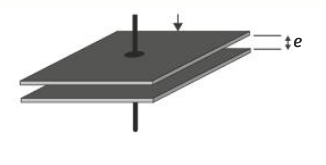
\includegraphics[scale=.7]{Ressources/TSPE_C11_AE1_Fig1.png}
		
		\columnbreak
		
		Pour une surface d'armatures $S$ = \num{10}\unit{\centi\meter\squared}\\
		
		\begin{tabular}{|c|c|c|c|c|c|}
			\hline \cellcolor{blue!30!white}$\mathbf{e}$ (\unit{\centi\meter})&0,1&0,2&0,5&1,0&5,0\\
			\hline \cellcolor{blue!30!white}$\mathbf{C}$ (\unit{\pico\farad})&8,8&4,4&1,8&0,9&0,3\\
			\hline
		\end{tabular}\\
	
		Pour une distance entre armatures $e$ = \num{1} \unit{\centi\meter}\\
		
		\begin{tabular}{|c|c|c|c|c|c|}
			\hline \cellcolor{blue!30!white}$\mathbf{S}$ (\unit{\centi\meter\squared})&1&5&10&40&100\\
			\hline \cellcolor{blue!30!white}$\mathbf{C}$ (\unit{\pico\farad})&0,09&0,4&0,9&3,5&8,9\\
			\hline
		\end{tabular}\\	
	\end{multicols}	
\end{minipage}}
\end{document}